\hyphenation{Schlei-cher}
\hyphenation{geo-me-try}

%\newcommand{\C}{\mathbb{C}}
%\newcommand{\R}{\mathbb{R}}

\subsubsection{Complex Dynamics }
\index{Schleicher, Dierk}

\paragraph{Research Team}

Dierk Schleicher (Professor), Alexandra Kaffl (PhD student, thesis
defense in July 2006), Johannes R\"uckert (PhD student, thesis
defense in July 2006), Nikita Selinger (PhD student).
%, Mihai
%Bailesteanu (Bachelor student). Non-scientific staff: Frauke
%Dammann, assistant for the International Mathematical Olympiad 2009,
%and a team of about 12 volunteers.

\medskip

%150 words or less -> shortened

Most of the research in my group is in complex dynamics: the
investigation of the dynamical system arising from iteration of a
holomorphic function $f\colon\C\to\C$, and questions from geometry
arising in this context. The particular strength of complex dynamics
comes from the fact that complex analysis provides powerful tools
for the study of dynamical systems, and the stiffness of complex
analysis often allows to answer many questions successfully in terms
of symbolic dynamics. A prominent and important example is the
dynamics of Newton's root-finding method.

%: if $g$ is a differentiable function (over the real or complex
%numbers), then the classical Newton method $N_g(z)=z-g(z)/g'(z)$ is
%often used to find zeroes of $g$  by iterating $N_{g}$. Even though
%Newton's method is as old as analysis, and extremely simple, it
Many questions are still open, especially about the global structure
of the basins of attraction for the various roots of $g$.
%There are
%a number of questions by Steve Smale (one of the fathers of the
%modern theory of dynamical systems); our work has helped to solve
%some of these questions.
Complex dynamics is an active research field that transcends
Newton's me\-thod. For polynomials, there is a classical theory by
Fatou and Julia (from the beginning of the 20-th century), by Douady
and Hubbard (from the 1980's), by Thurston and others. The theory of
transcendental functions is very different because many of the
successful tools for polynomials do not apply there. Much of our
research is related to bridging the gap from polynomials to
transcendental functions.
%Even for very special transcendental
%functions such as exponential functions, there are still unsolved
%fundamental questions: one recent result of my group is the complete
%answer to an extension of an old question by Euler.



\paragraph{Highlights}

{\em Our research team spent the spring semester 2006 at the Fields
Institute, Toronto, participating at the programme in Complex
Dynamics, Hyperbolic Geometry and Laminations.}


{\sl Dynamics of Newton's Method and R\"uckert's Thesis}.
One focus of the research in our group is Newton's method as a dynamical system on the complex plane. Newton's method is very easy to use and converges extremely fast near (simple) roots, but its global dynamical properties were poorly understood, which made it difficult to use in practice with guaranteed success. Figure~\ref{fig:prof_Schleicher} illustrates the complicated structure of the attracting basins of the various roots for a polynomial of degree $7$. Our general view is on understanding Newton's method as a dynamical system, not to compete with high-performance numerical algorithms. A survey on this point of view is appearing as \cite{JohannesNewtonSurvey}.

\begin{figure}[ht]
  \begin{center}
    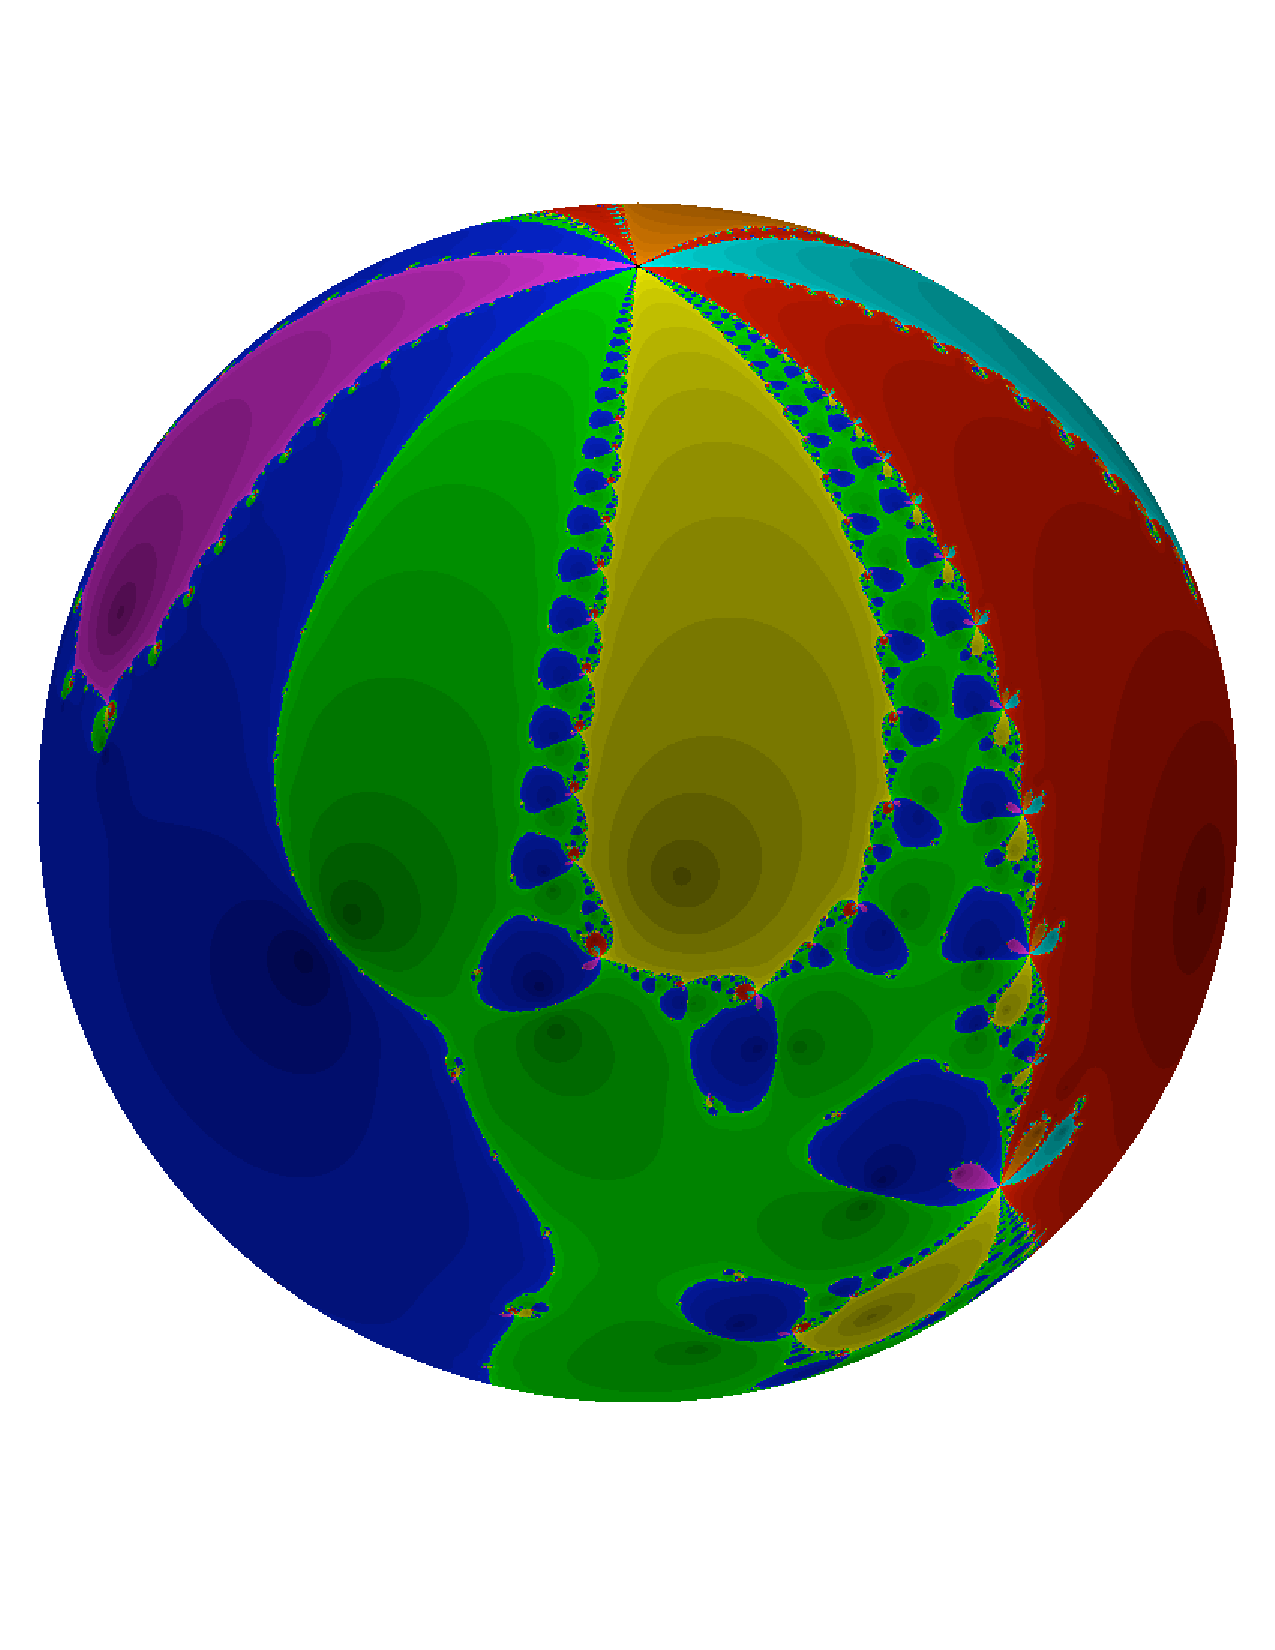
\includegraphics[width=6cm,viewport=018 120 600 700,clip]{Schleicher/Schleicher_2006_Fig1.pdf}
    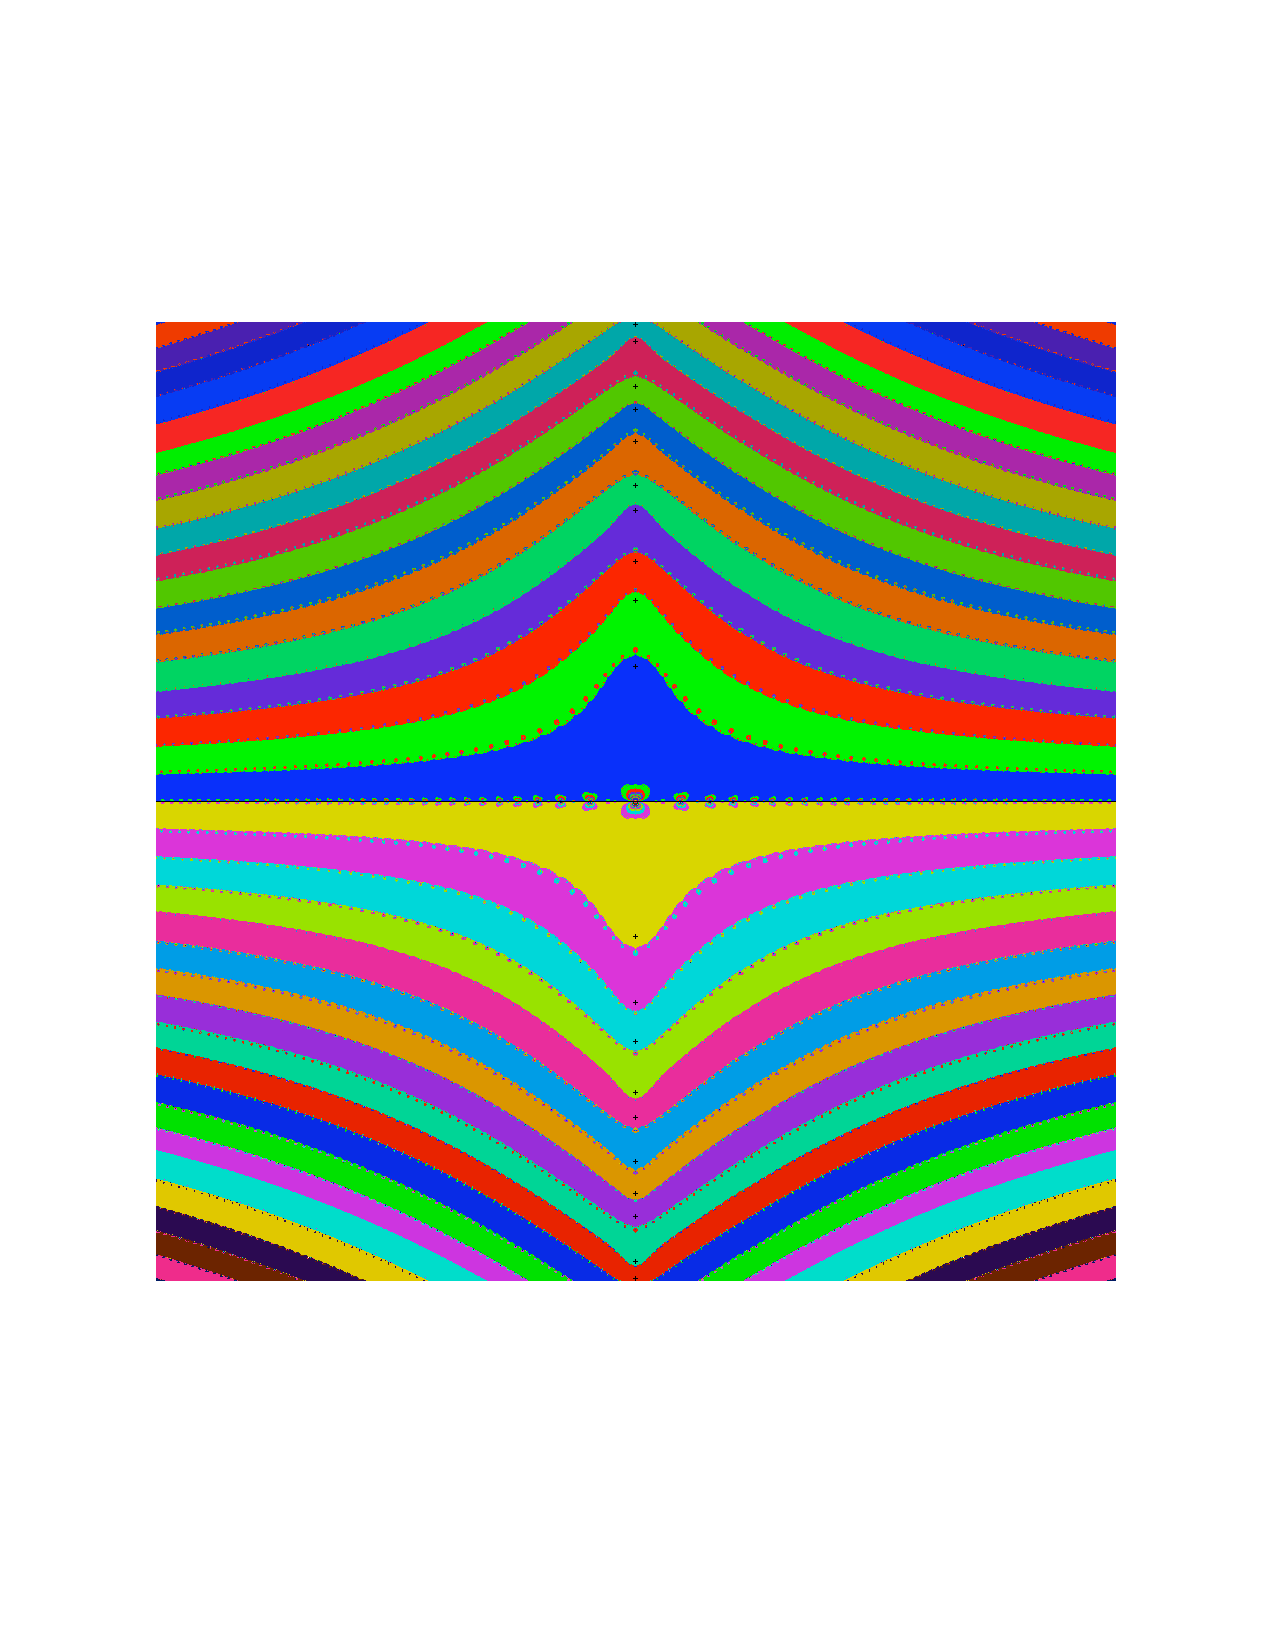
\includegraphics[width=6cm,viewport=050 180 530 630,clip]{Schleicher/Schleicher_2006_Fig2.pdf}
    \mycaption{ Top: Newton's method applied to a polynomial of degree $7$ in a single complex variable. Different colors indicate domains of attraction for the different roots. Bottom: Newton's method applied to the Riemann $\xi$ function: this is an entire transcendental function whose zeroes are exactly the non-trivial zeroes of the Riemann $\zeta$ function. }\label{fig:prof_Schleicher}
   \end{center}
\end{figure}
Recent results of our group include a good set of starting points for the Newton iteration: given only the degree $d$ of a complex polynomial and a trivial normalization, we can specify an explicit set $S_d$ of points so that starting Newton's method at these points is guaranteed to converge to all roots (joint with with Hubbard and Sutherland; Invent.\ Math.\ {\bf 146} (2001), 1--33); the number of points required is $O(d\log^2d)$. It was an open question how many iterations are required to find all roots with prescribed precision. We now managed to give an efficient bound on this number: it is essentially cubic in the degree $d$ and thus quite efficient \cite{NewtonOutline}. This made it possible to turn Newton's method for polynomials into an efficient algorithm with good complexity bounds.

We have made progress on extending these results to Newton's method for transcendental entire functions. A prime candidate is the Riemann $\xi$ function, an entire function the zeroes of which are exactly the non-trivial zeroes of the famous $\zeta$-function: see Figure~\ref{fig:prof_Schleicher} for an illustration and \cite{NewtonOutline} for some initial results. Three publications \cite{NewtonSebastian,BuffRueckert,NewtonEntire} study fundamental properties of Newton's method for arbitrary entire functions; a number of interesting similarities as well as differences to the polynomial case were discovered.

Finally, the difficult features of the Newton dynamics call for a classification of all possibilities, as proposed by Smale. This was achieved in \cite{NewtonJohannes} in an important special case. This result guides the way to a complete classification of (hyperbolic) Newton maps of polynomials; this is currently work in progress. An explicit classification of rational maps as dynamical systems is an important topic of current research; Newton maps would be the first such family (other than polynomials) that admits such a classification.
The study of Newton's method was the topic of the PhD thesis of Johannes R\"uckert~\cite{JohannesThesis}.

{\sl Symbolic Dynamics of Quadratic and Cubic Polynomials and Kaffl's thesis}.
Another focus of research in our group was symbolic dynamics related to iteration theory of polynomials. Polynomial dynamics is particularly successful because we have a variety of methods to describe their dynamics in terms of combinatorics and symbolic dynamics. With Bruin, we solved a number of the remaining open problems on the prototypical case of quadratic polynomials and started to collect old and new results in this area. Many of these results have been extended and generalized to ``unicritical'' polynomials of higher degrees by Alexandra Kaffl \cite{Alex1} in her PhD thesis~\cite{AlexThesis}, and jointly we finished this project into a monograph~\cite{SymDyn}.

Alexandra Kaffl managed to extend a number of these results from the case of one-dimensional parameter space (which by now is well understood) towards parameter spaces of dimension at least $2$ (a notoriously very difficult area). These results form another key part of her successful PhD thesis.

{\sl Further Research}.
A significant part of the research in our group is concerned with the dynamics of transcendental functions, either directly as dynamical systems \cite{ExpoSpiders, ExpoPSP,EscCosine, ExpoEscClass,ExpoBifComb,ExpoBif, ExpoParaRays}, from the point of view of Newton's method \cite{NewtonSebastian,BuffRueckert,NewtonEntire}, or in terms of Hausdorff dimension \cite{Cosine}, including a survey article \cite{Hausdorff} (see also the research report of 2005).

Finally, some research was inspired by mathematicians or mathematical topics from other areas \cite{Conway,FracSums}, including a publication on distortion-reduced color representation on screens and printers \cite{PhilippColor} that resulted from discussions with people from imaging science.


\goodbreak

\paragraph{Organization}
% list the (research) events you have organized, if any,

\begin{enumerate}
\item {\sl International Mathematical Olympiad (IMO) 2009.}
I continue to chair the local organizing committee for this event that will bring excellent students from around 100 countries to Bremen.
\item {\sl Deutsche Mathematik-Olympiaden e.V.}
In May, I was elected into the German Mathematical Olympiad Council (Vorstand des Deut\-sche Mathematik-Olympiaden e.V.).
\item {\sl Training to the German Team to the IMO 2006.}
Since Bremen was chosen as the site of the International Mathematical Olympiad 2009, Jacobs University Bremen has  become one of the training sites for the German team to the annual IMO's. Together with Michael Stoll and Alexei Belov, we have held the annual final training sessions before the IMO.
\item {\sl Studienstiftung des Deutschen Volkes.}
Since 2002, I have served as ``federf\"uhrender Vertrauensdozent'' for the ``Studienstiftung des Deut\-schen Volkes''; this appointment was renewed in 2006.

%\item

\end{enumerate}

\paragraph{Collaborations}
\begin{enumerate}
\item {\sl Univ.\ of Surrey, UK} \\
  Dr.~H. Bruin and A. Kaffl \\
  {\em Symbolic dynamics of quadratic polynomials}, joint monograph
\item {\sl Cornell University, NY/USA} \\
  Prof.~J. Hubbard \\
  Thurston theory for postsingularly finite exponential maps
\item {\sl Kyoto University, Japan} \\
  Prof.~M. Shishikura \\
  Thurston theory for postsingularly finite exponential maps
\item {\sl University of Liverpool} \\
  Dr.~L. Rempe \\
  Dynamics of transcendental functions, in particular complex exponential maps
\item {\sl Technische Universit\"at Berlin} \\
  M. M\"uller \\
  Summation with non-integer number of terms
\end{enumerate}


\paragraph{Grants}
% list the running grants in 2005, if none have been received, please delete this
% subsection.
\begin{enumerate}
\item Funded by State of Bremen, \emph{Continued Support for
Preparation of IMO 2009.} More funding expected 2007--2009 by the
Federal Republic of Germany and further sponsors. \item Funded by
Konrad-Adenauer-Stiftung, \emph{ support for graduate student
Alexandra Kaffl during her entire graduate education and in
particular for her stay at the Fields Institute, Toronto.} \item
Funded by Fields Institute \emph{membership as senior researcher
and travel support for Dierk Schleicher; full support for graduate
student Nikita Selinger; partial support for graduate student
Johannes R\"uckert}, (January-May 2006) \item Funded by Deutscher
Akademischer Austauschdienst \emph{support for graduate Johannes
R\"uckert during his stay at the Fields Institute, Toronto} \item
Funded by European Union, Marie Curie Research Training Network
FP6, \emph{Conformal structures and dynamics'' (CODY), network of
10 European countries, member of the German node and coordinator
of IUB involvement.} \item Funded by European Science Foundation,
\emph{ESF Research Networking Programmes ``Harmonic and complex
analysis and its applications'', network of 10 European countries;
member of the steering committee and coordinator of the German
node} (funding to be confirmed). \item Funded by Mathematisches
Forschungszentrum Oberwolfach \emph{co-organizer of a conference
``Trends and Developments in Complex Dynamics'' (with
Lyubich/Stony Brook, Petersen/Roskilde and Smillie/Cornell)}
conference proposal accepted, expenses sponsored by Oberwolfach.
%\item {Funded by}
\end{enumerate}

\paragraph{Awards, Prizes}
% list the grants you have received in 2005, if none have been received, please delete this % subsection.
\begin{enumerate}
\item {\sl Centro Internazionale Matematico
Estivo} in Cetraro, Cosenza, Italy, invited to offer course at
summer school in 2008.
%\item {\sl Bundeswettbewerb ``Jugend
%forscht'':} high school student Simon Schmitt from Bremen
%participated at the German youth science fair ``Jugend forscht
%2006''. First prize at the Bremen state level, federal award for the
%best interdisciplinary project, (Bundes\-sieger-Sonderpreis f\"ur
%die beste interdisziplin\"are Arbeit), sponsored by federal minister
%for education and research, Dr.~Annette Schavan. Advisor and mentor
%of this project was D.~Schleicher.
\end{enumerate}


% %{\bf Published in 2006}

% \bibitem{NewtonSebastian}
% Sebastian Mayer and Dierk Schleicher,
% {\em  Immediate and Virtual Basins of Newton's Method for Entire
% Functions}. {\em Annales de l'institut
% Fourier} {\bf 56} 2 (2006), 325--336. ArXiv math.DS/0403336.

% \bibitem{BuffRueckert}
% Xavier Buff and Johannes R\"uckert:
% {\em Virtual Immediate Basins of Newton Maps and Asymptotic Values}.
% {\em International Mathematics Research Notices}, Article ID 65498 (2006), 1--18.


% \bibitem{Conway}
% Dierk Schleicher and Michael Stoll,
% {\em An Introduction to Conway's Games and Numbers}. {\em Moscow Mathematics Journal}, {\bf 6} 2 (2006). ArXiv math.CO/0410026.





% {\bf Accepted for Publication in 2006}

% \bibitem{Cosine}
% Dierk Schleicher,
% {\em The dynamical fine structure of iterated cosine maps and a
% dimension paradox} (2005). {\em Duke Math Journal}, to appear. ArXiv math.DS/0406255.

% \bibitem{ExpoPSP}
% Bastian Laubner, Dierk Schleicher, Vlad Vicol,
% {\em A Combinatorial Classification of Postsingularly Preperiodic Complex Exponential Maps}
%  (2006). {\em Discrete and Continuous Dynamical Systems}, to appear. ArXiv math.DS/0602602.

% \bibitem{ExpoEscClass}
% Markus F\"orster, Dierk Schleicher, Lasse Rempe,
% {\em Classification of Escaping Exponential Maps}  (2004). ArXiv math.DS/0311427.



% {\bf In Publication}

% \bibitem {Hausdorff}
% Dierk Schleicher,
% {\em Hausdorff dimension, its properties,  and its surprises}.
% {\em American Mathematical Monthly}, to appear. ArXiv
% math.DS/0505099.

% \bibitem{ExpoBifComb}
% Lasse Rempe, Dierk Schleicher, {\em Combinatorics of bifurcations in exponential parameter space},
% ArXiv math.DS/0408011.
% Invited for a volume of Cambridge University Press in memory of
% Noel Baker (Phil Rippon, ed).

% \bibitem{EscCosine}
% G\"unter Rottenfu{\ss}er,
% {\em Escaping Points of the Cosine Family},
%  ArXiv math.DS/0403012. To appear in a volume of
% Cambridge University Press in memory of Noel Baker (Phil Rippon,
% ed.).

% \bibitem{Alex1}
% Alexandra Kaffl,
% {\em On the Structure of Abstract Hubbard Trees and the Space of Abstract
% Kneading Sequences of Degree Two}. To appear in: {\em Ergodic Theory and
% Dynamical Systems}.


% {\bf Submitted and under Review}


% \bibitem{ExpoBif}
% Lasse Rempe, Dierk Schleicher,
% {\em Bifurcations in the Space of Exponential Maps} (2004).
% Preprint Nr.~3, Institute for Mathematical Sciences at Stony Brook
% (2004). ArXiv math.DS/0311480.

% \bibitem{ExpoParaRays}
% Markus F\"orster, Dierk Schleicher,
% {\em Parameter rays for the complex exponential family} (2005). ArXiv math.DS/050597.

% \bibitem {ExpoSpiders}
% John Hubbard, Dierk Schleicher, Mitsuhiro Shishikura,
% {\em A Topological Characterization of Postsingularly Finite
% Exponential Maps and Limits of Quadratic Differentials}. Manuscript (2006), submitted.

% \bibitem{NewtonJohannes}
% Johannes R\"uckert, {\em Combinatorial structure of immediate basins of Newton maps} (2005).

% \bibitem{NewtonEntire}
%  Johannes R\"uckert, Dierk Schleicher,
% {\em On Newton's method for entire functions} (2005).
% ArXiv math.DS/0505652.

% \bibitem{NewtonOutline}
% Dierk Schleicher,
% {\em Newton's method is efficient as a dynamical system for polynomials}.
% Manuscript, Proceedings of the Fields Institute, Toronto (2006).

% \bibitem{JohannesNewtonSurvey}
% Johannes R\"uckert, {\em Rational and Transcendental Newton Maps}.
% Preprint, Proceedings of the Fields Institute, Toronto (2006).





% \bibitem{SymDyn}
% Henk Bruin, Alexandra Kaffl, Dierk Schleicher,
% {\it Symbolic Dynamics of Quadratic Polynomials}.
% Monograph, to be published; 221 pages. (An earlier version appeared as a report of the
% Institute Mittag-Leffler, Djursholm {\bf 7} (2001/02) ).

% \bibitem {FracSums}
% Markus M\"uller, Dierk Schleicher,
% {\em Fractional Sums and Euler-like Identities} (2005). ArXiv math.CA/0502109.




% \bibitem{PhilippColor}
% Philipp Urban, Mitchell R.\ Rosen, Roy S.\ Berns, Dierk Schleicher,
% {\em Embedding non-euclidean color spaces into euclidean color spaces
% with minimal isometric disagreement}. Manuscript, submitted.

% {\bf PhD Theses}

% \bibitem{AlexThesis}
% Alexandra Kaffl,
% {\em Hubbard trees and kneading sequences for unicritical and quadratic polynomials}. PhD thesis, International University Bremen (2006). External Reviewers: Milnor (Stony Brook), Rees (Liverpool).

% \end{thebibliography}
